\documentclass{standalone}
\usepackage{tikz}
\usetikzlibrary{patterns, positioning}


\begin{document}
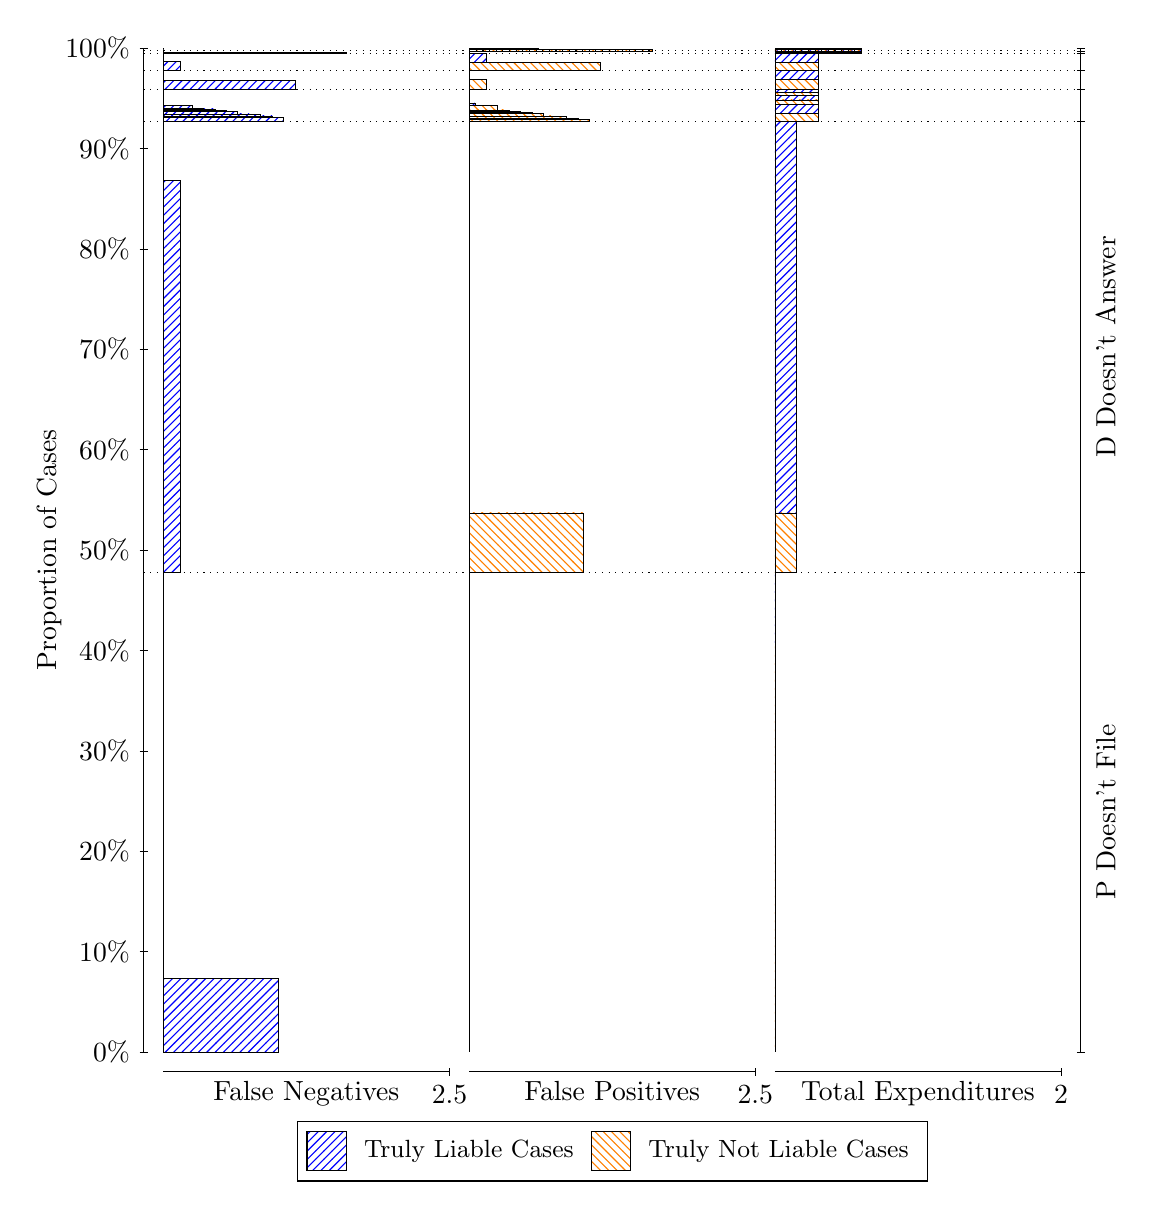
\begin{tikzpicture}
\draw[black, very thin] (1.5,1.75) -- (1.5,14.5);
\node[rotate=90, text=black, anchor=center] at (0.3, 8.125) {Proportion of Cases};
\draw[black, very thin] (1.45,1.75) -- (1.55,1.75);
\node[text=black, anchor=east] at (1.45, 1.75) {0\%};
\draw[black, very thin] (1.45,3.025) -- (1.55,3.025);
\node[text=black, anchor=east] at (1.45, 3.025) {10\%};
\draw[black, very thin] (1.45,4.3) -- (1.55,4.3);
\node[text=black, anchor=east] at (1.45, 4.3) {20\%};
\draw[black, very thin] (1.45,5.575) -- (1.55,5.575);
\node[text=black, anchor=east] at (1.45, 5.575) {30\%};
\draw[black, very thin] (1.45,6.85) -- (1.55,6.85);
\node[text=black, anchor=east] at (1.45, 6.85) {40\%};
\draw[black, very thin] (1.45,8.125) -- (1.55,8.125);
\node[text=black, anchor=east] at (1.45, 8.125) {50\%};
\draw[black, very thin] (1.45,9.4) -- (1.55,9.4);
\node[text=black, anchor=east] at (1.45, 9.4) {60\%};
\draw[black, very thin] (1.45,10.675) -- (1.55,10.675);
\node[text=black, anchor=east] at (1.45, 10.675) {70\%};
\draw[black, very thin] (1.45,11.95) -- (1.55,11.95);
\node[text=black, anchor=east] at (1.45, 11.95) {80\%};
\draw[black, very thin] (1.45,13.225) -- (1.55,13.225);
\node[text=black, anchor=east] at (1.45, 13.225) {90\%};
\draw[black, very thin] (1.45,14.5) -- (1.55,14.5);
\node[text=black, anchor=east] at (1.45, 14.5) {100\%};

\draw[black, very thin] (13.4,1.75) -- (13.4,14.5);
\draw[black, very thin] (13.35,1.75) -- (13.45,1.75);
\node[anchor=west] at (13.35, 1.75) {};
\draw[black, very thin] (13.35,7.8437) -- (13.45,7.8437);
\node[anchor=west] at (13.35, 7.8437) {};
\draw[black, very thin] (13.35,13.569) -- (13.45,13.569);
\node[anchor=west] at (13.35, 13.569) {};
\draw[black, very thin] (13.35,13.973) -- (13.45,13.973);
\node[anchor=west] at (13.35, 13.973) {};
\draw[black, very thin] (13.35,14.212) -- (13.45,14.212);
\node[anchor=west] at (13.35, 14.212) {};
\draw[black, very thin] (13.35,14.431) -- (13.45,14.431);
\node[anchor=west] at (13.35, 14.431) {};
\draw[black, very thin] (13.35,14.465) -- (13.45,14.465);
\node[anchor=west] at (13.35, 14.465) {};
\draw[black, very thin] (13.35,14.5) -- (13.45,14.5);
\node[anchor=west] at (13.35, 14.5) {};

\draw[black, very thin, pattern color=blue, pattern=north east lines] (1.75,1.75) rectangle (3.2033,2.6873);
\draw[black, very thin, pattern color=orange, pattern=north west lines] (1.75,2.6873) rectangle (1.75,7.8437);
\draw[black, very thin, pattern color=blue, pattern=north east lines] (1.75,7.8437) rectangle (1.968,12.816);
\draw[black, very thin, pattern color=orange, pattern=north west lines] (1.75,12.816) rectangle (1.75,13.569);
\draw[black, very thin, pattern color=blue, pattern=north east lines] (1.75,13.569) rectangle (3.276,13.622);
\draw[black, very thin, pattern color=blue, pattern=north east lines] (1.75,13.622) rectangle (3.1307,13.637);
\draw[black, very thin, pattern color=blue, pattern=north east lines] (1.75,13.637) rectangle (2.9853,13.656);
\draw[black, very thin, pattern color=blue, pattern=north east lines] (1.75,13.656) rectangle (2.84,13.665);
\draw[black, very thin, pattern color=blue, pattern=north east lines] (1.75,13.665) rectangle (2.6947,13.698);
\draw[black, very thin, pattern color=blue, pattern=north east lines] (1.75,13.698) rectangle (2.5493,13.707);
\draw[black, very thin, pattern color=blue, pattern=north east lines] (1.75,13.707) rectangle (2.404,13.726);
\draw[black, very thin, pattern color=blue, pattern=north east lines] (1.75,13.726) rectangle (2.2587,13.737);
\draw[black, very thin, pattern color=blue, pattern=north east lines] (1.75,13.737) rectangle (2.1133,13.77);
\draw[black, very thin, pattern color=orange, pattern=north west lines] (1.75,13.77) rectangle (1.75,13.973);
\draw[black, very thin, pattern color=blue, pattern=north east lines] (1.75,13.973) rectangle (3.4213,14.086);
\draw[black, very thin, pattern color=orange, pattern=north west lines] (1.75,14.086) rectangle (1.75,14.212);
\draw[black, very thin, pattern color=blue, pattern=north east lines] (1.75,14.212) rectangle (1.968,14.328);
\draw[black, very thin, pattern color=orange, pattern=north west lines] (1.75,14.328) rectangle (1.75,14.431);
\draw[black, very thin, pattern color=blue, pattern=north east lines] (1.75,14.431) rectangle (4.0753,14.446);
\draw[black, very thin, pattern color=orange, pattern=north west lines] (1.75,14.446) rectangle (1.75,14.465);
\draw[black, very thin, pattern color=orange, pattern=north west lines] (1.75,14.465) rectangle (1.75,14.479);
\draw[black, very thin, pattern color=blue, pattern=north east lines] (1.75,14.479) rectangle (1.75,14.5);
\draw[black, very thin, pattern color=orange, pattern=north west lines] (5.6333,1.75) rectangle (5.6333,6.9064);
\draw[black, very thin, pattern color=blue, pattern=north east lines] (5.6333,6.9064) rectangle (5.6333,7.8437);
\draw[black, very thin, pattern color=orange, pattern=north west lines] (5.6333,7.8437) rectangle (7.0867,8.5972);
\draw[black, very thin, pattern color=blue, pattern=north east lines] (5.6333,8.5972) rectangle (5.6333,13.569);
\draw[black, very thin, pattern color=orange, pattern=north west lines] (5.6333,13.569) rectangle (7.1593,13.597);
\draw[black, very thin, pattern color=orange, pattern=north west lines] (5.6333,13.597) rectangle (7.014,13.609);
\draw[black, very thin, pattern color=orange, pattern=north west lines] (5.6333,13.609) rectangle (6.8687,13.628);
\draw[black, very thin, pattern color=orange, pattern=north west lines] (5.6333,13.628) rectangle (6.7233,13.637);
\draw[black, very thin, pattern color=orange, pattern=north west lines] (5.6333,13.637) rectangle (6.578,13.67);
\draw[black, very thin, pattern color=orange, pattern=north west lines] (5.6333,13.67) rectangle (6.4327,13.674);
\draw[black, very thin, pattern color=orange, pattern=north west lines] (5.6333,13.674) rectangle (6.4327,13.679);
\draw[black, very thin, pattern color=orange, pattern=north west lines] (5.6333,13.679) rectangle (6.2873,13.698);
\draw[black, very thin, pattern color=orange, pattern=north west lines] (5.6333,13.698) rectangle (6.142,13.713);
\draw[black, very thin, pattern color=orange, pattern=north west lines] (5.6333,13.713) rectangle (5.9967,13.772);
\draw[black, very thin, pattern color=blue, pattern=north east lines] (5.6333,13.772) rectangle (5.706,13.804);
\draw[black, very thin, pattern color=blue, pattern=north east lines] (5.6333,13.804) rectangle (5.6333,13.973);
\draw[black, very thin, pattern color=orange, pattern=north west lines] (5.6333,13.973) rectangle (5.8513,14.098);
\draw[black, very thin, pattern color=blue, pattern=north east lines] (5.6333,14.098) rectangle (5.6333,14.212);
\draw[black, very thin, pattern color=orange, pattern=north west lines] (5.6333,14.212) rectangle (7.3047,14.315);
\draw[black, very thin, pattern color=blue, pattern=north east lines] (5.6333,14.315) rectangle (5.8513,14.431);
\draw[black, very thin, pattern color=orange, pattern=north west lines] (5.6333,14.431) rectangle (5.6333,14.45);
\draw[black, very thin, pattern color=blue, pattern=north east lines] (5.6333,14.45) rectangle (5.6333,14.465);
\draw[black, very thin, pattern color=orange, pattern=north west lines] (5.6333,14.465) rectangle (7.9587,14.479);
\draw[black, very thin, pattern color=blue, pattern=north east lines] (5.6333,14.479) rectangle (6.5053,14.5);
\draw[black, very thin, pattern color=orange, pattern=north west lines] (9.5167,1.75) rectangle (9.5167,6.9064);
\draw[black, very thin, pattern color=blue, pattern=north east lines] (9.5167,6.9064) rectangle (9.5167,7.8437);
\draw[black, very thin, pattern color=orange, pattern=north west lines] (9.5167,7.8437) rectangle (9.7892,8.5972);
\draw[black, very thin, pattern color=blue, pattern=north east lines] (9.5167,8.5972) rectangle (9.7892,13.569);
\draw[black, very thin, pattern color=orange, pattern=north west lines] (9.5167,13.569) rectangle (10.062,13.674);
\draw[black, very thin, pattern color=blue, pattern=north east lines] (9.5167,13.674) rectangle (10.062,13.783);
\draw[black, very thin, pattern color=orange, pattern=north west lines] (9.5167,13.783) rectangle (10.062,13.842);
\draw[black, very thin, pattern color=blue, pattern=north east lines] (9.5167,13.842) rectangle (10.062,13.895);
\draw[black, very thin, pattern color=orange, pattern=north west lines] (9.5167,13.895) rectangle (10.062,13.934);
\draw[black, very thin, pattern color=blue, pattern=north east lines] (9.5167,13.934) rectangle (10.062,13.973);
\draw[black, very thin, pattern color=orange, pattern=north west lines] (9.5167,13.973) rectangle (10.062,14.098);
\draw[black, very thin, pattern color=blue, pattern=north east lines] (9.5167,14.098) rectangle (10.062,14.212);
\draw[black, very thin, pattern color=orange, pattern=north west lines] (9.5167,14.212) rectangle (10.062,14.315);
\draw[black, very thin, pattern color=blue, pattern=north east lines] (9.5167,14.315) rectangle (10.062,14.431);
\draw[black, very thin, pattern color=orange, pattern=north west lines] (9.5167,14.431) rectangle (10.607,14.45);
\draw[black, very thin, pattern color=blue, pattern=north east lines] (9.5167,14.45) rectangle (10.607,14.465);
\draw[black, very thin, pattern color=orange, pattern=north west lines] (9.5167,14.465) rectangle (10.607,14.479);
\draw[black, very thin, pattern color=blue, pattern=north east lines] (9.5167,14.479) rectangle (10.607,14.5);
\draw[black, dotted] (1.5,7.8437) -- (13.4,7.8437);
\draw[black, dotted] (1.5,13.569) -- (13.4,13.569);
\draw[black, dotted] (1.5,13.973) -- (13.4,13.973);
\draw[black, dotted] (1.5,14.212) -- (13.4,14.212);
\draw[black, dotted] (1.5,14.431) -- (13.4,14.431);
\draw[black, dotted] (1.5,14.465) -- (13.4,14.465);
\draw[black, very thin] (1.75,1.5) -- (5.3833,1.5);
\node[text=black, anchor=north] at (3.5667, 1.5) {False Negatives};
\draw[black, very thin] (5.3833,1.45) -- (5.3833,1.55);
\node[text=black, anchor=north] at (5.3833, 1.45) {2.5};

\draw[black, very thin] (5.6333,1.5) -- (9.2667,1.5);
\node[text=black, anchor=north] at (7.45, 1.5) {False Positives};
\draw[black, very thin] (9.2667,1.45) -- (9.2667,1.55);
\node[text=black, anchor=north] at (9.2667, 1.45) {2.5};

\draw[black, very thin] (9.5167,1.5) -- (13.15,1.5);
\node[text=black, anchor=north] at (11.333, 1.5) {Total Expenditures};
\draw[black, very thin] (13.15,1.45) -- (13.15,1.55);
\node[text=black, anchor=north] at (13.15, 1.45) {2};

\node[text=black, centered, rotate=90] at (13.72, 4.7969) {P Doesn't File};
\node[text=black, centered, rotate=90] at (13.72, 10.706) {D Doesn't Answer};






\draw (7.449999999999999,1.5) node[draw=none] (baseCoordinate) {};
\begin{scope}[align=center]
        \matrix[scale=0.5, draw=black, below=0.5cm of baseCoordinate, nodes={draw}, column sep=0.1cm]{
            \node[rectangle, draw, minimum width=0.5cm, minimum height=0.5cm, pattern color=blue, pattern=north east lines] {}; &
            \node[draw=none, font=\small, text=black] (B) {Truly Liable Cases}; &
            \node[rectangle, draw, minimum width=0.5cm, minimum height=0.5cm, pattern color=orange, pattern=north west lines] {}; &
            \node[draw=none, font=\small, text=black] (B) {Truly Not Liable Cases}; \\
            };
\end{scope}

\end{tikzpicture}
\end{document}